\chapter{Int\'egration des \'equations du mouvement}

\section{Mouvement lin\'eaire}

L'\'equation (\ref{EQ:5_5}) appliqu\'ee \`a un point mat\'eriel donne en coordonn\'ees g\'en\'eralis\'ees :
\be
	L = \frac{1}{2}a(q)\dot{q}^{2} - U(q) \label{EQ:11_1}
\ee
qui s'\'ecrit en coordonn\'ees cart\'esiennes :
\be
	L = \frac{1}{2}m\dot{x}^{2} - U(x) \label{EQ:11_2}
\ee
En \'ecrivant l'\'energie totale :
\bea
	E = T + U & = & \frac{1}{2}m\dot{x}^{2} + U(x) \nonumber \\
	\dot{x}^{2} & = & \frac{2}{m}(E-U(x)) \nonumber \\
	\dfrac{\mathrm{d}x}{\mathrm{dt}} & = & \sqrt{\frac{2}{m}(E-U(x))} \nonumber \\
	t & = & \sqrt{\frac{m}{2}}\int{\dfrac{\mathrm{d}x}{\sqrt{E-U(x)}}} + cste \label{EQ:11_3}
\eea
o\`u $E$ et $cste$ sont des constantes du mouvement, la premi\`ere par la loi de conservation de l'\'energie et la seconde par int\'egration.

Lors d'un mouvement, l'\'energie totale est toujours sup\'erieure \`a l'\'energie potentielle car l'\'energie cint\'etique ne peut \^etre n\'egative. Aussi le mouvement ne peut \^etre possible que si $U(x)<E$.

\begin{figure}[htb!]
	\begin{center}
		\begin{picture}(200,150)(0,0)
			%axis
			\linethickness{0.05mm}
			\put(0,0){\line(1,0){200}}\put(202,-2){$x$}
			\put(0,0){\line(0,1){140}}\put(-2,142){$U$}
			%curve
			\linethickness{0.5mm}
			\qbezier(-5,130),(15,130),(25,110)
			\qbezier(25,110),(35,90),(55,90)
			\qbezier(55,90),(80,90),(90,100)
			\qbezier(90,100),(100,110),(125,110)
			\qbezier(125,110),(150,110),(190,20)
			%limit
			\linethickness{0.05mm}
			\multiput(-5,100)(10,0){20}{\line(1,0){8}}\put(195,98){$U=E$}
			\multiput(32,0)(0,5){20}{\line(0,1){3}}\put(34,102){$A$}\put(28,-7){$x_{1}$}
			\multiput(90,0)(0,5){20}{\line(0,1){3}}\put(82,102){$B$}\put(86,-7){$x_{2}$}
			\put(142,102){$C$}
		\end{picture}
		\caption{Exemple d'une fonction d\'efinissant l'\'energie potentielle}\label{FIG:3_1}
	\end{center}
\end{figure}

Sur la figure (\ref{FIG:3_1}), la condition $U(x)<E$ implique que le mouvement n'est possible que sur les intervalles tels que $x\in\left[A\,;B\right]$ et $x\in\left[C\,;+\infty\right[$. Dans le premier cas, le mouvement est dit fini et oscillatoire. Dans le second cas, le mouvement est dit inifini. Les points tels que :
\be
	U(x) = E \label{EQ:11_4}
\ee
sont les \emph{points d'arr\^et}. En effet, dans ce cas, l'\'energie cin\'etique du point mat\'eriel est nulle car sa vitesse aussi de facto.

Dans la relation (\ref{EQ:5_1}), nous avons vu que le temps n'est pas qu'uniforme, il est aussi isotrope. Ainsi la transformation $\mathrm{t}\mapsto -\mathrm{t}$ laisse inchang\'ee la fonction de Lagrange et les \'equations du mouvement. Ainsi $\Delta\mathrm{t}(x_{1}\rightarrow x_{2}) = \Delta\mathrm{t}(x_{2}\rightarrow x_{1})$ et la période d'oscillation $\mathrm{T}(E)=\Delta\mathrm{t}(x_{1}\rightarrow x_{2}\rightarrow x_{1})$ vaut $2\Delta\mathrm{t}(x_{1}\rightarrow x_{2})$. L'\'equation (\ref{EQ:11_3}) s'\'ecrit alors :
\bea
	\mathrm{T}(E) & = & 2\sqrt{\frac{m}{2}}\int_{x_{1}(E)}^{x_{2}(E)}{\dfrac{\mathrm{d}x}{\sqrt{E-U(x)}}} \nonumber \\
	\mathrm{T}(E) & = & \sqrt{2m}\int_{x_{1}(E)}^{x_{2}(E)}{\dfrac{\mathrm{d}x}{\sqrt{E-U(x)}}}\label{EQ:11_5}
\eea
qui d\'etermine la p\'eriode d'oscillation de la particule mat\'erielle en fonction de son \'energie totale.

\section{D\'efinition de l'\'energie potentielle en fonction de la p\'eriode des oscillations}

\begin{figure}[htb!]
	\begin{center}
		\begin{picture}(200,150)(0,0)
			%axis
			\linethickness{0.05mm}
			\put(0,0){\line(1,0){200}}\put(202,-2){$x$}
			\put(100,0){\line(0,1){140}}\put(98,142){$U$}
			%curve
			\linethickness{0.5mm}
			\qbezier(35,120),(40,0),(100,0)
			\qbezier(100,0),(175,0),(180,120)
			\put(47,50){$x_{1}(U)$}
			\put(132,50){$x_{2}(U)$}
			%limit
			\linethickness{0.05mm}
			\multiput(-5,80)(10,0){20}{\line(1,0){8}}\put(195,78){$U=E$}
			\multiput(40,0)(0,5){16}{\line(0,1){3}}\put(35,-7){$x_{1}$}
			\multiput(175,0)(0,5){16}{\line(0,1){3}}\put(170,-7){$x_{2}$}
		\end{picture}
		\caption{Fonction d\'efinissant l'\'energie potentielle ayant qu'un unique minimum}\label{FIG:3_2}
	\end{center}
\end{figure}

L'objectif de ce paragraphe est de trouver la fonction d\'efinissant l'\'energie potentielle d'un champ $U$ connaissant la p\'eriode d'oscillations $\mathrm{T}(E)$ du mouvement animant une particule. Pour cela, nous supposons que la fonction recherch\'ee $U$ n'a qu'un unique minimum dans la r\'egion du mouvement et que, comme sur la figure (\ref{FIG:3_2}), $U(0) = 0$.

Transformons l'int\'egrale (\ref{EQ:11_5}) avec $x$ fonction de $U$ telle que pour une valeur de l'\'energie potentielle $U$ il existe deux valeurs de $x$ diff\'erentes. Elle devient alors la somme de deux int\'egrales sur deux r\'egions diff\'erentes :
\bea
	\mathrm{T}(E) & = & \sqrt{2m}\int_{x_{1}(E)}^{x_{2}(E)}\dfrac{\mathrm{d}x}{\sqrt{E - U(x)}} \nonumber \\
	& = & -\sqrt{2m}\int_{0}^{E}\dfrac{\mathrm{d}x_{1}}{\mathrm{d}U}\dfrac{\mathrm{d}U}{\sqrt{E - U}} + \sqrt{2m}\int_{0}^{E}\dfrac{\mathrm{d}x_{2}}{\mathrm{d}U}\dfrac{\mathrm{d}U}{\sqrt{E - U}} \nonumber \\
	& = & \sqrt{2m}\int_{0}^{E}\left[\dfrac{\mathrm{d}x_{2}}{\mathrm{d}U} - \dfrac{\mathrm{d}x_{1}}{\mathrm{d}U}\right]\dfrac{\mathrm{d}U}{\sqrt{E - U}}
\eea
Elle peut \^etre \'etendue \`a :
\bea
	\int_{0}^{\alpha}\dfrac{\mathrm{T}(E)\mathrm{d}E}{\sqrt{\alpha - E}} & = & \sqrt{2m}\int_{0}^{\alpha}\int_{0}^{E}\left[\dfrac{\mathrm{d}x_{2}}{\mathrm{d}U} - \dfrac{\mathrm{d}x_{1}}{\mathrm{d}U}\right]\dfrac{\mathrm{d}U\mathrm{d}E}{\sqrt{(\alpha - E)(E - U)}} \nonumber \\
	& =& \sqrt{2m}\int_{0}^{\alpha}\left[\dfrac{\mathrm{d}x_{2}}{\mathrm{d}U} - \dfrac{\mathrm{d}x_{1}}{\mathrm{d}U}\right]\mathrm{d}U\int_{U}^{\alpha}\dfrac{\mathrm{d}E}{\sqrt{(\alpha - E)(E - U)}}
\eea
La seconde implication dans sa deuxi\`eme int\'egrale est en $\int_{U}^{\alpha}$ car en dehors de cet intervalle, $\int_{0}^{U}$ et $\int_{\alpha}^{E}$ sont ind\'efinie car $(E-U)$ et $(\alpha-E)$ sont respectivement n\'egatives.

Faisons d\'esormais le calcul de la seconde int\'egrale, soit :
\be
	\int_{U}^{\alpha}\dfrac{\mathrm{d}E}{\sqrt{(\alpha - E)(E - U)}}
\ee
en posant :
\be
	y = \dfrac{2E - U - \alpha}{\alpha - U}
\ee
qui donne :
\be
	\begin{cases}
		E = \dfrac{(\alpha - U)y + U + \alpha}{2} \\
		\mathrm{d}y = \dfrac{2\mathrm{d}E}{\alpha - U} \Leftrightarrow \mathrm{d}E = \dfrac{\alpha - U}{2}\mathrm{d}y
	\end{cases}
\ee
et :
\be
	\begin{cases}
		E = U \Rightarrow y = \dfrac{U - \alpha}{\alpha - U} = -1 \\
		E = \alpha \Rightarrow y = \dfrac{-U + \alpha}{\alpha - U} = 1
	\end{cases}
\ee
Ainsi :
\bea
	\int_{U}^{\alpha}\dfrac{\mathrm{d}E}{\sqrt{(\alpha - E)(E - U)}} & = & \int_{-1}^{1}\dfrac{(\alpha - U)\mathrm{d}y}{2\sqrt{\frac{(2\alpha - (\alpha - U)y + U + \alpha)}{2}\frac{((\alpha - U)y + U + \alpha - 2U)}{2}}} \nonumber \\
	& = & \int_{-1}^{1}\dfrac{(\alpha - U)\mathrm{d}y}{2\sqrt{\frac{(\alpha - U - (\alpha - U)y)}{2}\frac{(\alpha - U + (\alpha - U)y)}{2}}} \nonumber \\
	& = & \int_{-1}^{1}\dfrac{(\alpha - U)\mathrm{d}y}{2\frac{\alpha - U}{2}\sqrt{(1 - y)(1 + y)}} \nonumber \\
	& = & \int_{-1}^{1}\dfrac{\mathrm{d}y}{\sqrt{1 - y^{2}}}
\eea
En posant $u = y^{2}$ soit $y = u^{1/2}$ et $\mathrm{d}u = 2y\mathrm{d}y = 2u^{1/2}\mathrm{d}y \Leftrightarrow \mathrm{d}y = \frac{1}{2}u^{-1/2}\mathrm{d}u$, l'int\'egrale pr\'ec\'edente s'\'ecrit :
\bea
	\int_{U}^{\alpha}\dfrac{\mathrm{d}E}{\sqrt{(\alpha - E)(E - U)}} & = & \int_{-1}^{1}\dfrac{\mathrm{d}y}{\sqrt{1 - y^{2}}} \nonumber \\
	& = & 2 \int_{0}^{1}\dfrac{1}{2}\dfrac{u^{-1/2}\mathrm{d}u}{(1-u)^{1/2}} \nonumber \\
	& = & \int_{0}^{1}u^{-1/2}(1-u)^{-1/2}\mathrm{d}u \nonumber \\
	& = & \mathrm{B}\left(\frac{1}{2},\frac{1}{2}\right) = \dfrac{\Gamma(\frac{1}{2})\Gamma(\frac{1}{2})}{\Gamma(1)} = \pi
\eea
De fait :
\bea
	\int_{0}^{\alpha}\dfrac{\mathrm{T}(E)\mathrm{d}E}{\sqrt{\alpha - E}} & = & \sqrt{2m}\pi\int_{0}^{\alpha}\left[\dfrac{\mathrm{d}x_{2}}{\mathrm{d}U} - \dfrac{\mathrm{d}x_{1}}{\mathrm{d}U}\right]\mathrm{d}U \nonumber \\
	& = & \sqrt{2m}\pi\left[x_{2}(\alpha) - x_{2}(0) - x_{1}(\alpha) + x_{1}(0)\right]
\eea
Or par hypoth\`ese, $x_{2}(0) = x_{1}(0) = 0$, donc :
\be
	\int_{0}^{\alpha}\dfrac{\mathrm{T}(E)\mathrm{d}E}{\sqrt{\alpha - E}} = \sqrt{2m}\pi\left[x_{2}(\alpha) - x_{1}(\alpha)\right]
\ee
Dans le cas o\`u nous posons $\alpha = U$, nous pouvons en d\'eduire :
\be
	x_{2}(U) - x_{1}(U) = \dfrac{1}{\sqrt{2m}\pi}\int_{0}^{U}\dfrac{\mathrm{T}(E)\mathrm{d}E}{\sqrt{U - E}} \label{EQ:12_1}
\ee
De plus, si le champ d'\'energie potentielle est paire tel que $U(x) = U(-x)$ ou encore $x_{1}(U) = -x_{2}(U) = x(U)$, alors l'\'equation (\ref{EQ:12_1}) devient, puisque $x_{2}(U) - x_{1}(U) = 2x(U)$ :
\be
	x(U) = \dfrac{1}{2\pi\sqrt{2m}}\int_{0}^{U}\dfrac{\mathrm{T}(E)\mathrm{d}E}{\sqrt{U - E}} \label{EQ:12_2}
\ee

\section{Masse r\'eduite}

L'important probl\`eme du mouvement s'un syst\`eme ferm\'e \`a deux particules r\'eagissant l'une sur l'autre, ou encore \emph{probl\`eme des deux corps}, admet une solution g\'en\'erale compl\`ete. Pour le r\'esoudre, nous allons le simplifier en d\'ecomposant le mouvement du syst\`eme en celui du centre d'inertie et des deux points mat\'eriels par rapport \`a ce dernier. L'\'energie potentielle d'int\'eraction ne d\'epend que de la distance entre les deux particules, aussi la fonction de Lagrange s'\'ecrit :
\be
	L = \dfrac{m_{1}\dot{r}_{1}^{2}}{2} + \dfrac{m_{2}\dot{r}_{2}^{2}}{2} - U(\lvert \vec{r}_{1} - \vec{r}_{2} \rvert) \label{EQ:13_1}
\ee
D\'efinissons $\vec{r} = \vec{r}_{1} - \vec{r}_{2}$ et pla\c{c}ons l'origine des coordonn\'ees au centre d'inertie. Alors l'\'equation (\ref{EQ:8_3}) donne $\vec{R} = \vec{0}$ ou encore : $\sum m_{a}\vec{r}_{a} = \vec{0}$, soit :
\be
	m_{1}\vec{r}_{1} + m_{2}\vec{r}_{2} = \vec{0}
\ee
Nous pouvons en conclure que :
\be
	\vec{r} = \begin{cases}
		\vec{r}_{1} + \dfrac{m_{1}}{m_{2}}\vec{r}_{1} = \dfrac{m_{1} + m_{2}}{m_{2}}\vec{r}_{1} \\
		- \dfrac{m_{2}}{m_{1}}\vec{r}_{2} - \vec{r}_{2} = -\dfrac{m_{1} + m_{2}}{m_{1}}\vec{r}_{2}
	\end{cases}
\ee
soit :
\be
	\begin{cases}
		\vec{r}_{1} = \dfrac{m_{2}}{m_{1} + m_{2}}\vec{r} \\
		\vec{r}_{2} = \dfrac{-m_{1}}{m_{1} + m_{2}}\vec{r}
	\end{cases}\label{EQ:13_2}
\ee
Puisque :
\be
	\begin{cases}
		\vec{\dot{r}}_{1} = \dfrac{m_{2}}{m_{1} + m_{2}}\vec{\dot{r}} \\
		\vec{\dot{r}}_{2} = \dfrac{-m_{1}}{m_{1} + m_{2}}\vec{\dot{r}}
	\end{cases}
\ee
la fonction de Lagrange se d\'eveloppe ainsi :
\bea
	L & = & \dfrac{m_{1}}{2}\left(\dfrac{m_{2}}{m_{1} + m_{2}}\right)^{2}\vec{\dot{r}}^{\,2} + \dfrac{m_{2}}{2}\left(\dfrac{-m_{1}}{m_{1} + m_{2}}\right)^{2}\vec{\dot{r}}^{\,2} - U(\vec{r}) \nonumber \\
	& = & \dfrac{m_{1}m_{2}^{2} + m_{1}^{2}m_{2}}{2(m_{1} + m_{2})^{2}}\vec{\dot{r}}^{\,2} - U(\vec{r}) \nonumber \\
	& = & \dfrac{m_{1}m_{2}(m_{2} + m_{1})}{2(m_{1} + m_{2})^{2}}\vec{\dot{r}}^{\,2} - U(\vec{r})
\eea
et on peut conclure en posant \emph{la masse r\'eduite} :
\be
	m = \dfrac{m_{1}m_{2}}{(m_{1} + m_{2})} \label{EQ:13_4}
\ee
\`a :
\be
	L = \dfrac{m}{2}\vec{\dot{r}}^{\,2} - U(\vec{r}) \label{EQ:13_3}
\ee
qui est la fonction de Lagrange d'un point mat\'eriel de masse $m$ se d\'epla\c{c}ant dans le champ ext\'erieur $U(\vec{r})$ qui est sym\'etrique par rapport au point immobile des coordonn\'ees, soit le centre d'inertie. Ainsi le calcul de $\vec{r} = \vec{r}(\mathrm{t})$ permet gr\^ace aux \'equations (\ref{EQ:13_2}) d'en d\'eduire les trajectoires $\vec{r}_{1}(\mathrm{t})$ et $\vec{r}_{2}(\mathrm{t})$ des particules de masse respective $m_{1}$ et $m_{2}$.

\section{Mouvement dans un champ central}

Le fait de ramener le probl\`eme \`a deux corps \`a celui d'un seul nous conduit \`a devoir d\'eterminer le mouvement d'une particule dans un champ ext\'erieur o\`u son \'energie potentielle ne d\'epend que de la distance $r$ \`a un point immobile. Ce champ est appel\'e \emph{champ central}. De la relation (\ref{EQ:5_4}), la force est donn\'ee par :
\be
	\vec{F} = -\dfrac{\partial U(r)}{\partial\vec{r}} = -\dfrac{\mathrm{d}U(r)}{\mathrm{d}r}\dfrac{\vec{r}}{r}
\ee
et agissant sur la particule, elle ne d\'epend aussi que de $r$.

Par d\'efinition, \'equation (\ref{EQ:9_3}), le moment cin\'etique est :
\be
	\vec{M} = \vec{r}\wedge\vec{p}
\ee
et dans un champ central, il se conserve dans un r\'ef\'erentiel dont un axe passe par le centre et ce dernier est le centre du r\'ef\'erentiel. Dans ce cas de conservation et parce que $\vec{M}\perp\vec{p}$ alors le mouvement de la particule reste toujours dans le m\^eme plan perpendiculaire au moment cin\'etique. Ainsi, en coordonn\'ees polaires (cylindriques), nous avons de facto $\dot{z} = 0$ et la fonction de Lagrange est, voir l'\'equation (\ref{EQ:4_5}) :
\be
	L = \dfrac{m}{2}(\dot{r}^{2} + r^{2}\dot{\varphi}^{2}) - U(r) \label{EQ:14_1}
\ee
La coordonn\'ee $\varphi$ est dite \emph{cyclique} car elle n'appara\^it pas explicitement dans la d\'efinition de la fonction de Lagrange, alors que $r$ et $\dot{\varphi}$ en sont des coordonn\'ees \emph{principales}. Pour la coordonn\'ee $\varphi$, les \'equations de Lagrange (\ref{EQ:2_6}) sont :
\be
	\dfrac{\mathrm{d}}{\mathrm{dt}}\left(\dfrac{\partial L}{\partial\dot{q}_{i}}\right) = \dfrac{\partial L}{\partial q_{i}} = 0
\ee
Ainsi, l'impulsion g\'en\'eralis\'ee, \'equation (\ref{EQ:7_5}) :
\be
	p_{i} = \dfrac{\partial L}{\partial\dot{q}_{i}}
\ee
est constante dans le temps, i.e. $p_{i}$ est une int\'egrale premi\`ere, soit une int\'egrale du mouvement qui conserve sa valeur pendant le mouvement. L'\'equation (\ref{EQ:14_1}) permet d'\'ecrire\footnote{Il s'agit bien de $p_{\varphi}$ et non pas de $\dot{p}_{\varphi}$ commme inscrit dans le livre.} :
\be
	\dfrac{\partial L}{\partial\dot{q}_{i}} = mr^{2}\dot{\varphi} = p_{\varphi}
\ee
et la valeur de $p_{\varphi}$ se conserve dans le temps. En appliquant l'\'equation (\ref{EQ:9_7}) car nous avons choisi le r\'ef\'erentiel tel que la particule tourne dans un plan perpendiculaire \`a un axe passant par le centre du champ :
\bea
	M_{z} & = & \dfrac{\partial L}{\partial\dot{\varphi}_{i}} \nonumber \\
	\Leftrightarrow M & = & mr^{2}\dot{\varphi} \label{EQ:14_2}
\eea
Car les valeurs de $M$ et de $M_{z}$ se confondent par d\'efinition du choix fait pr\'ec\'edemment. La valeur de $M$ est donc conserv\'ee \'egalement. $\dot{\varphi}$ ne changeant pas de signe au cours du mouvement\footnote{En effet, $M$ est une valeur constante, commme $m$ alors que $r^{2}$ est toujours positive.}, $\varphi$ \'evolue de mani\`ere monotone.

\begin{figure}[htb!]
	\begin{center}
		\begin{picture}(200,150)(0,0)
			%curve
			\linethickness{0.5mm}
			\qbezier(120,150),(150,125),(170,75)
			\qbezier(170,75),(180,50),(190,5)
			%vectors
			\linethickness{0.05mm}
			\put(-8,47){$0$}
			\put(0,50){\vector(1,0){178}}
			\put(75,80){$\vec{r}$}
			\put(0,50){\vector(8,2){163}}
			%tangent
			\multiput(162,50)(0,5){8}{\line(0,1){3}}
			\put(135,65){$r\mathrm{d}\varphi$}
			%angle
			\qbezier(25,50),(25,55),(20,55)
			\put(27,52){$\mathrm{d}\varphi$}
		\end{picture}
		\caption{Aire balay\'ee}\label{FIG:3_7}
	\end{center}
\end{figure}

R\'efl\'echissons d\'esormais à l'interpr\'etation g\'eom\'etrique de la loi pr\'ec\'edente (\ref{EQ:14_2}) en remarquant que l'expression $\frac{1}{2}\vec{r}\cdot\vec{r}\mathrm{d}\varphi$ repr\'sente la surface form\'ee par les deux rayons vecteurs infiniment voisins et l'arc de la trajectoire de la figure (\ref{FIG:3_9}). En d\'esignant par $\mathrm{d}f$ cet \'el\'ement de surface, le moment cin\'etique de la particule devient :
\be
	M = 2m\dot{f} \label{EQ:14_3}
\ee
car en s'aidant de la relation (\ref{EQ:14_2}) :
\bea
	\mathrm{d}f & = & \dfrac{1}{2}\vec{r}\cdot\vec{r}\mathrm{d}\varphi \nonumber \\
	& = & \dfrac{1}{2}r^{2}\mathrm{d}\varphi \nonumber \\
	\dot{f} = \dfrac{\mathrm{d}f}{\mathrm{dt}} & = & \dfrac{1}{2}r^{2}\dot{\varphi} \nonumber
\eea
La grandeur $\dot{f}$ est alors appel\'ee \emph{vitesse a\'erolaire}. Et comme le moment cin\'etique $M$ est constant pendant le mouvement alors la vitesse a\'erolaire est constante \'egalement, il s'agit de la \emph{seconde loi de Kepler}, \`a savoir que pendant des intervalles de temps \'egaux, le rayon vecteur d'un point mobile balaye des aires \'egales. Cette seconde loi est aussi appel\'ee \emph{int\'egrale des aires} qui est la loi de conservation du moment cin\'etique d'une particule en mouvement dans un champ central.

Pour obtenir la solution compl\`ete du mouvement d'une particule dans un champ central, utilisons les lois de conservation de l'\'energie (\'equation (\ref{EQ:6_1}) et du moment cin\'etique (\'equation (\ref{EQ:9_3}). D'apr\`es la relation (\ref{EQ:14_2}), $\dot{\varphi} = \frac{M}{mr^{2}}$, donc l'\'energie peut s'\'ecrire comme :
\be
	E = T + U = \dfrac{m}{2}(\dot{r}^{2} + r^{2}\dot{\varphi}^{2}) + U(r) = \dfrac{m}{2}\dot{r}^{2} + \dfrac{M^{2}}{2mr^{2}} + U(r) \label{EQ:14_4}
\ee
qui implique directement :
\be
	\dot{r} = \dfrac{\mathrm{d}r}{\mathrm{dt}} = \pm\sqrt{\frac{2}{m}(E - U(r)) - \frac{M^{2}}{m^{2}r^{2}}} \label{EQ:14_5}
\ee
En renversant, nous obtenons :
\be
	\mathrm{dt} = \dfrac{\mathrm{d}r}{\sqrt{\frac{2}{m}(E - U(r)) - \frac{M^{2}}{m^{2}r^{2}}}}
\ee
qui permet d'obtenir par intégration :
\be
	t = \int{\dfrac{\mathrm{d}r}{\sqrt{\frac{2}{m}(E - U(r)) - \frac{M^{2}}{m^{2}r^{2}}}}} + cste \label{EQ:14_6}
\ee

En reprenant l'\'equation (\ref{EQ:14_2}) sous la forme :
\bea
	M & = & mr^{2}\dot{\varphi} \nonumber \\
	\mathrm{d}\varphi & = & \dfrac{M}{mr^{2}}\mathrm{dt}
\eea
et en l'injection dans la relation (\ref{EQ:14_5}), nous avons :
\bea
	\dfrac{\mathrm{d}r}{\mathrm{dt}} = \dfrac{M\mathrm{d}r}{mr^{2}\mathrm{d}\varphi} & = & \sqrt{\frac{2}{m}(E - U(r)) - \frac{M^{2}}{m^{2}r^{2}}} \nonumber \\
	\Leftrightarrow \mathrm{d}\varphi & = & \dfrac{M\mathrm{d}r}{mr^{2}\sqrt{\frac{2}{m}(E - U(r)) - \frac{M^{2}}{m^{2}r^{2}}}} \nonumber \\
	& = & \dfrac{\frac{M}{r^{2}}\mathrm{d}r}{\sqrt{2m(E - U(r)) - \frac{M^{2}}{r^{2}}}} \nonumber \\
	\Leftrightarrow \varphi & = & \int{\dfrac{\frac{M}{r^{2}}\mathrm{d}r}{\sqrt{2m(E - U(r)) - \frac{M^{2}}{r^{2}}}}} + cste \label{EQ:14_7}
\eea

Les formules (\ref{EQ:14_6}) et (\ref{EQ:14_7}) forment la solution g\'en\'erale. La premi\`ere donne implicitement la distance au centre $r$ en fonction du temps alors que la seconde \'etablit la relation entre $r$ et $\varphi$, soit l'\'equation du mouvement.

\begin{figure}[htb!]
	\begin{center}
		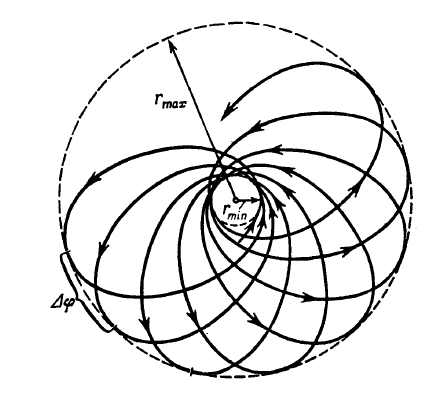
\includegraphics[width=10cm]{chapter_03_paragraph_14_fig_09}
		\caption{Trajectoire dans un champ central}\label{FIG:3_9}
	\end{center}
\end{figure}

L'\'equation (\ref{EQ:14_4}) :
\be
	E = T + U = \dfrac{m}{2}\dot{r}^{2} + \dfrac{M^{2}}{2mr^{2}} + U(r)
\ee
peut se r\'e\'ecrire en identifiant $\frac{m}{2}\dot{r}^{2}$ comme l'\'energie cin\'etique radiale de la particule comme :
\be
	E = \dfrac{m}{2}\dot{r}^{2} + U_{\mathrm{eff}}(r)
\ee
avec :
\be
	U_{\mathrm{eff}}(r) = \dfrac{M^{2}}{2mr^{2}} + U(r) \label{EQ:14_8}
\ee
se d\'efinissant comme une \'energie potentielle efficace o\`u le terme $\frac{M^{2}}{2mr^{2}}$ est l'\emph{\'energie centrifuge}. Ainsi, la partie radiale du mouvement de la particule peut \^etre consid\'er\'ee comme un mouvement lin\'eaire dans un champ dot\'e d'une \'energie potentielle efficace.

Les valeurs de la distance telle que l'\'energie cin\'etique radiale s'annule ou encore $E = U_{\mathrm{eff}}(r)$ d\'elimitent le domaine du mouvement de la particule car cela n\'ecessite de facto $\dot{r} = 0$. Cela d\'efinit les \emph{points de rebroussement} o\`u la particule peut encore avoir une vitesse angulaire $\dot{\varphi}\neq 0$. La fonction $r(\mathrm{t})$ devient ensuite croissante ou d\'ecroissante. Il existe alors deux possibilit\'es :
\begin{itemize}
	\item $r \gg r_{min}$ alors le mouvement est infini
	\item $r_{min} \leqslant r \leqslant r_{max}$ alors la trajectoire est contenue dans l'anneau d\'efini par les cercles de rayon $r_{min}$ et $r_{max}$
\end{itemize}
Dans le second cas, la variation angulaire $\Delta\varphi$ de la trajectoire de la particule pendant qu'elle fait le trajet $r_{max} \rightarrow r_{min} \rightarrow r_{max}$\footnote{Ou l'\'equivalent sym\'etrique $r_{min} \rightarrow r_{max} \rightarrow r_{min}$.} vaut d'apr\`es l'\'equation (\ref{EQ:14_7}) :
\be
	\Delta\varphi = 2\int_{r_{min}}^{r_{max}}{\dfrac{\frac{M}{r^{2}}\mathrm{d}r}{\sqrt{2m(E - U(r)) - \frac{M^{2}}{r^{2}}}}} \label{EQ:14_10}
\ee
La trajectoire de la particule est finie, i.e. elle se referme, si et seulement si $\Delta\varphi = \frac{m}{n}\times 2\pi$ avec ${m;n}\in\mathbb{N}$. Ainsi, quand le rayon vecteur parcourt $n$ p\'eriodes, il fait \'egalement $m$ tours complets et la trajectoire se referme. Toutefois, cela reste un cas particulier. En g\'en\'eral $U(r)$ ne permet par d'obtenir $\Delta\varphi$ comme une fraction rationnelle de $2\pi$ et la trajectoire ne se referme pas et finit par remplir tout l'espace de l'anneau compris entre $r_{min}$ et $r_{max}$. Finalement, la trajectoire est ferm\'ee pour les \'energies potentielles en $\frac{1}{r}$, voir le paragraphe \ref{PAR:15} et en $r^{2}$, voir l'exercice \ref{EX:5_14}.

Aux points de rebroussement d\'efinis tels que $\dot{r} = 0$, il y a un changement de signe de la vitesse radiale et donc de la direction radiale prise par la particule. Que ce soit en $r_{min}$ ou $r_{max}$, la quantit\'e $\dfrac{\dot{r}(\mathrm{t} - \delta\mathrm{t})}{\dot{r}(\mathrm{t} + \delta\mathrm{t})}$ est n\'egative. La trajectoire est ainsi sym\'etrique par rapport \`a la direction indiqu\'ee.

Pour le mouvement d'une particule ayant une moment cin\'etique non nulle, la position $r=0$ est inatteignable car :
\be
	\lim_{r\rightarrow 0}\dfrac{M^{2}}{2mr^{2}} \rightarrow +\infty
\ee

L'\'equation (\ref{EQ:14_4}) implique de facto\footnote{Dans l'expression finale de cette s\'equence, le livre affiche le signe $<$ au lieu de $>$.} :
\bea
	E - U(r) - \dfrac{M^{2}}{2mr^{2}} & = & \dfrac{m\dot{r}^{2}}{2} > 0 \nonumber \\
	r^{2}E - r^{2}U(r) & > & \dfrac{M^{2}}{2m} \nonumber \\
	r^{2}E & > & r^{2}U(r) + \dfrac{M^{2}}{2m}
\eea

Par conservation de l'\'energie, nous avons si $\lim_{r\rightarrow 0} r^{2}E = 0$, aussi $r$ ne peut tendre vers 0 que si :
\bea
	0 & > & \lim_{r\rightarrow 0}(r^{2}U(r)) + \dfrac{M^{2}}{2mr^{2}} \nonumber \\
	\lim_{r\rightarrow 0}(r^{2}U(r)) & < & -\dfrac{M^{2}}{2mr^{2}} \label{EQ:14_11}
\eea
Et cette derni\`ere in\'egalit\'e n'est vraie que dans deux situations et implique que $r$ peut ainsi tendre vers le centre du champ d'\'energie potentielle :
\begin{itemize}
	\item $U(r)=\dfrac{-\alpha}{r^{2}}$ avec $\alpha > \dfrac{M^{2}}{2mr^{2}}$
	\item $U(r)=\dfrac{-\alpha}{r^{n}}$ avec $n > 2$ car $\lim_{r\rightarrow 0}(r^{2}U(r)) = \lim_{r\rightarrow 0}\left(\dfrac{-\alpha}{r^{n-2}}\right) = -\infty < -\dfrac{M^{2}}{2mr^{2}}$
\end{itemize}

\section{Le probl\`eme de Kepler}\label{PAR:15}